\documentclass[10pt,conference]{IEEEtran}
% Conference mode locks out \IEEEaftertitletext, which places Fig. 1 between the title and the abstract.
\IEEEoverridecommandlockouts

\usepackage[T1]{fontenc}
\usepackage[utf8]{inputenc}
\usepackage{amsmath,amssymb}
\usepackage{graphicx}
\usepackage{booktabs}
\usepackage{xcolor}
\usepackage{pifont}
\usepackage{listings}
\usepackage{tikz}
\usetikzlibrary{arrows.meta}
\usepackage{capt-of}
\usepackage{cite}
\usepackage[hidelinks]{hyperref}
\usepackage{xurl}
\hypersetup{
  pdftitle={Teralizer: A Tool for Generalizing JUnit Tests into Property-Based jqwik Tests},
  pdfauthor={Johann Glock, Clemens Bauer, Martin Pinzger},
  pdflang={en-US}
}

\newcommand{\Teralizer}{\textsc{Teralizer}}
% Code uses Latin Modern Typewriter, which is narrower than the Courier of the class.
\newcommand{\codefont}{\fontfamily{lmtt}\selectfont}
\newcommand{\code}[1]{{\codefont #1}}
\newcommand{\runin}[1]{\textit{#1:}}
\newcommand{\Naive}{\textsc{Naive}}
\newcommand{\Improved}{\textsc{Improved}}

\lstdefinestyle{code}{
  basicstyle=\codefont\fontsize{7.6}{9}\selectfont,
  columns=fullflexible,
  keepspaces=true,
  showstringspaces=false,
  aboveskip=4pt,
  belowskip=4pt,
  xleftmargin=1em
}

% The output of the example run in Fig. 3. Hyphens stay hyphens, so that the columns of the tables line up.
\lstdefinestyle{console}{
  basicstyle=\codefont\fontsize{5.5}{6.6}\selectfont,
  columns=fullflexible,
  keepspaces=true,
  showstringspaces=false,
  literate={-}{{-}}1,
  frame=single,
  framerule=0.4pt,
  framesep=2pt,
  rulecolor=\color{black!22},
  backgroundcolor=\color{black!2},
  xleftmargin=2.4pt,
  xrightmargin=2.4pt,
  aboveskip=0pt,
  belowskip=2pt
}

% Colors and styles of the figures. Blue marks what stems from the path condition and orange what stems from
% the symbolic output. Red and green mark the removed and the added lines of the refactoring in Fig. 1, and
% their darker shades the condition that it changes.
\definecolor{inhl}{RGB}{212,227,247}
\definecolor{outhl}{RGB}{253,224,190}
\definecolor{delhl}{RGB}{250,214,214}
\definecolor{addhl}{RGB}{212,239,212}
\definecolor{delmark}{RGB}{240,168,168}
\definecolor{addmark}{RGB}{158,214,158}
% A highlight inside a line of code that does not widen the line.
\newcommand{\slip}[2]{\hspace{-\fboxsep}\colorbox{#1}{#2}\hspace{-\fboxsep}}
\definecolor{effone}{RGB}{13,122,120}
\definecolor{efften}{RGB}{52,84,160}
\definecolor{effsixty}{RGB}{194,65,12}
\tikzset{
  paperfig/.style={x=1pt, y=1pt, font=\sffamily,
    execute at begin picture={\setlength{\fboxsep}{1.2pt}},
    panel/.style={draw=black!30, line width=0.5pt, rounded corners=2.5pt, fill=white},
    subbox/.style={draw=black!22, line width=0.4pt, rounded corners=1.5pt, fill=black!2},
    num/.style={circle, fill=black, text=white, inner sep=0pt, minimum size=8.2pt,
      font=\sffamily\bfseries\fontsize{5.8}{6}\selectfont},
    ttl/.style={anchor=base west, yshift=-2.5pt, inner sep=0pt, font=\sffamily\bfseries\fontsize{7.1}{8.1}\selectfont},
    code/.style={anchor=west, inner sep=0pt, font=\fontfamily{lmtt}\fontsize{5.7}{6.9}\selectfont},
    txt/.style={anchor=west, inner sep=0pt, font=\sffamily\fontsize{6.0}{7.1}\selectfont},
    tag/.style={anchor=west, inner sep=0pt, font=\sffamily\fontsize{5.7}{6.7}\selectfont},
    hdr/.style={txt, font=\sffamily\bfseries\fontsize{5.7}{6.7}\selectfont, text=black!65},
    spec/.style={anchor=west, inner xsep=2.5pt, inner ysep=1.6pt, rounded corners=1.2pt,
      font=\sffamily\fontsize{6.2}{7.2}\selectfont},
    badge/.style={tag, line width=0.3pt, rounded corners=1.2pt, inner xsep=2.5pt, inner ysep=1.2pt},
    flow/.style={-{Triangle[length=3.0pt, width=4.6pt]}, line width=1.0pt, black!60}
  }
}

\title{Teralizer: A Tool for Generalizing JUnit Tests\\into Property-Based jqwik Tests}

\author{%
\IEEEauthorblockN{Johann Glock}
\IEEEauthorblockA{\textit{Software Competence Center}\\
\textit{Hagenberg (SCCH)}\\
Hagenberg, Austria\\
0000-0002-0152-8611}
\and
\IEEEauthorblockN{Clemens Bauer}
\IEEEauthorblockA{\textit{Department of Informatics Systems}\\
\textit{University of Klagenfurt}\\
Klagenfurt, Austria\\
0009-0000-9199-8563}
\and
\IEEEauthorblockN{Martin Pinzger}
\IEEEauthorblockA{\textit{Department of Informatics Systems}\\
\textit{University of Klagenfurt}\\
Klagenfurt, Austria\\
0000-0002-5536-3859}}

% Fig. 1 spans both columns below the author block. It is built once in a box.
\newsavebox{\ideabox}
\IEEEaftertitletext{%
  \setbox\ideabox=\vbox{%
    \vspace*{-0.4\baselineskip}%
    {\centering% Fig. 1: test generalization with Teralizer on the test fullApproval of the running example, drawn at
% the full text width of IEEEtran conference papers (516 pt). A Source comment stands above each panel.
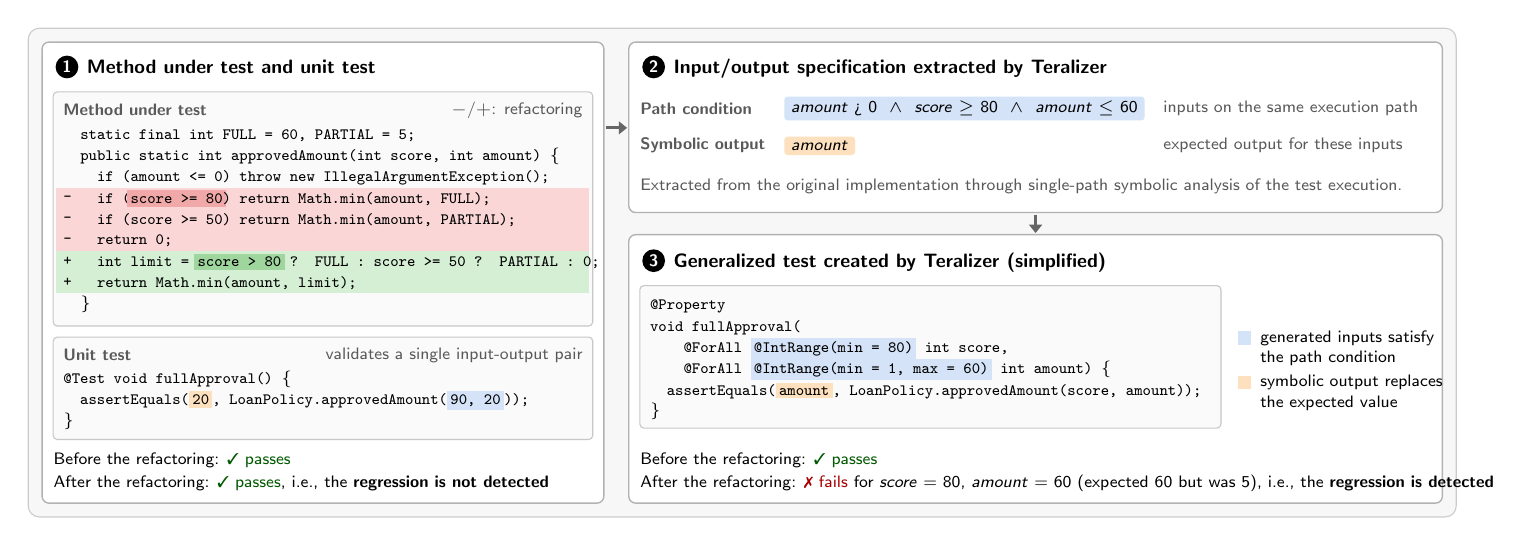
\begin{tikzpicture}[paperfig]
\draw[rounded corners=4pt, fill=black!3, draw=black!20, line width=0.4pt] (0,0) rectangle (516,-176.6);
\draw[panel] (5,-5) rectangle (208,-171.6);
\draw[panel] (217,-5) rectangle (511,-66.6);
\draw[panel] (217,-74.6) rectangle (511,-171.6);
\draw[flow] (208.8,-36) -- (216.4,-36);
\draw[flow] (364,-67.4) -- (364,-74);

% (1) the method under test with the refactoring, and the unit test
% Source: demo/loan/src/main/java/bank/LoanPolicy.java (lines 4 to 11) for the method, and
% demo/loan/src/test/java/bank/LoanPolicyTest.java (lines 8 to 10) for the test. The removed lines are
% lines 8 to 10 of that method, and the added lines are lines 8 and 9 of demo/refactoring/LoanPolicy.java,
% with which demo/run.sh replaces the method. The darker boxes mark the condition that the refactoring
% changes. demo/output/regression.txt shows that the three original tests pass after the refactoring.
\node[num] at (14,-14) {1};
\node[ttl] at (21,-14) {Method under test and unit test};

\draw[subbox] (9,-23) rectangle (204,-107.6);
\node[hdr] at (12.5,-29.5) {Method under test};
\node[tag, anchor=east, text=black!65] at (200.5,-29.5) {$-$/$+$: refactoring};
\fill[delhl] (10.2,-80.6) rectangle (202.8,-57.8);
\fill[addhl] (10.2,-95.8) rectangle (202.8,-80.6);
\foreach \y in {-61.6, -69.2, -76.8} \node[code] at (12.5,\y) {-};
\foreach \y in {-84.4, -92.0} \node[code] at (12.5,\y) {+};
\node[code] at (18.6,-38.8) {static final int FULL = 60, PARTIAL = 5;};
\node[code] at (18.6,-46.4) {public static int approvedAmount(int score, int amount) \{};
\node[code] at (18.6,-54.0) {\ \ if (amount <= 0) throw new IllegalArgumentException();};
\node[code] at (18.6,-61.6) {\ \ if (\slip{delmark}{score >= 80}) return Math.min(amount, FULL);};
\node[code] at (18.6,-69.2) {\ \ if (score >= 50) return Math.min(amount, PARTIAL);};
\node[code] at (18.6,-76.8) {\ \ return 0;};
\node[code] at (18.6,-84.4) {\ \ int limit = \slip{addmark}{score > 80} ? FULL : score >= 50 ? PARTIAL : 0;};
\node[code] at (18.6,-92.0) {\ \ return Math.min(amount, limit);};
\node[code] at (18.6,-99.6) {\}};

\draw[subbox] (9,-111.6) rectangle (204,-148.6);
\node[hdr] at (12.5,-118.1) {Unit test};
\node[tag, anchor=east, text=black!65] at (200.5,-118.1) {validates a single input-output pair};
\node[code] at (12.5,-127.0) {@Test void fullApproval() \{};
\node[code] at (12.5,-134.6) {\ \ assertEquals(\colorbox{outhl}{20}, LoanPolicy.approvedAmount(\colorbox{inhl}{90, 20}));};
\node[code] at (12.5,-142.2) {\}};

\node[tag] at (9,-156.1) {Before the refactoring: \textcolor{green!35!black}{\ding{51}\ passes}};
\node[tag] at (9,-164.6) {After the refactoring: \textcolor{green!35!black}{\ding{51}\ passes}, i.e., the \textbf{regression is not detected}};

% (2) the specification that Teralizer extracts
% Source: demo/output/specs/bank.LoanPolicyTest.fullApproval.2.jpf.symbolic.input.json (the path
% condition) and ...symbolic.output.json (the symbolic output), and
% sections/02-background.tex of the Teralizer paper (Symbolic Analysis for Specification Extraction)
% for what the two elements describe and how they are extracted.
\node[num] at (226,-14) {2};
\node[ttl] at (233,-14) {Input/output specification extracted by \Teralizer{}};

\node[hdr] at (221,-29) {Path condition};
\node[spec, fill=inhl] at (273,-29) {\textit{amount} > 0 \ $\land$\ \ \textit{score} $\ge$ 80 \ $\land$\ \ \textit{amount} $\le$ 60};
\node[tag, text=black!65] at (410,-29) {inputs on the same execution path};
\node[hdr] at (221,-42.5) {Symbolic output};
\node[spec, fill=outhl] at (273,-42.5) {\textit{amount}};
\node[tag, text=black!65] at (410,-42.5) {expected output for these inputs};
\node[tag, text=black!65] at (221,-57) {Extracted from the original implementation through single-path symbolic analysis of the test execution.};

% (3) the generalized test and what it detects
% Source: demo/output/generated/_LoanPolicyTest_Generalized_fullApproval_2_Test.java. The panel shows
% the test method (lines 345 to 351) in simplified form: the ranges that TestParametersSupplier
% (lines 367 to 405) implements are written as jqwik annotations, and the parameter object, the
% package qualifiers and the recording of the tested inputs are left out. The two results are those of
% demo/output/adoption.txt (passes for the original implementation) and demo/output/regression.txt
% (fails after the refactoring).
\node[num] at (226,-84) {3};
\node[ttl] at (233,-84) {Generalized test created by \Teralizer{} (simplified)};

\draw[subbox] (221,-93) rectangle (431,-144.5);
\node[code] at (224.5,-100.6) {@Property};
\node[code] at (224.5,-108.2) {void fullApproval(};
\node[code] at (224.5,-115.8) {\ \ \ \ @ForAll \colorbox{inhl}{@IntRange(min = 80)} int score,};
\node[code] at (224.5,-123.4) {\ \ \ \ @ForAll \colorbox{inhl}{@IntRange(min = 1, max = 60)} int amount) \{};
\node[code] at (224.5,-131.0) {\ \ assertEquals(\colorbox{outhl}{amount}, LoanPolicy.approvedAmount(score, amount));};
\node[code] at (224.5,-138.6) {\}};

\fill[inhl] (437,-114.5) rectangle (442,-109.5);
\node[tag] at (445,-112) {generated inputs satisfy};
\node[tag] at (445,-119.4) {the path condition};
\fill[outhl] (437,-130.5) rectangle (442,-125.5);
\node[tag] at (445,-128) {symbolic output replaces};
\node[tag] at (445,-135.4) {the expected value};

\node[tag] at (221,-156.1) {Before the refactoring: \textcolor{green!35!black}{\ding{51}\ passes}};
\node[tag] at (221,-164.6) {After the refactoring: \textcolor{red!65!black}{\ding{55}\ fails} for \textit{score} = 80, \textit{amount} = 60 (expected 60 but was 5), i.e., the \textbf{regression is detected}};
\end{tikzpicture}
\par}%
    \vspace{0.3\baselineskip}%
    % Source: the sources that figures/idea.tex names for its three panels
    \captionof{figure}{Test generalization with \Teralizer{} on the running example. (1)~The unit test validates a single input and passes before and after a refactoring that unintentionally changes the condition \code{score >= 80} to \code{score > 80}. (2)~\Teralizer{} extracts the path condition and the symbolic output expression of the tested execution path. (3)~The generalized test validates the assertion for generated inputs that satisfy the path condition and thereby detects the regression.}%
    \label{fig:idea}}%
  \nointerlineskip\box\ideabox\vspace*{\baselineskip}}

\begin{document}

\maketitle

\begin{abstract}
% Source: the abstract and sections/01-introduction.tex of the Teralizer paper
\textbf{Background:} Property-based testing validates properties across many generated inputs and can thereby detect regressions that conventional unit tests miss.
However, writing property-based tests is challenging for practitioners, which limits their adoption.
% Source: the abstract of the Teralizer paper (main.tex, Objective and Design)
\textbf{Tool:} \Teralizer{} automatically generalizes JUnit tests into property-based jqwik tests for regression detection.
Through single-path symbolic analysis, it extracts from each test execution a path condition, which characterizes the inputs that follow the same execution path, and a symbolic output expression, which computes the expected output for these inputs.
The generalized tests generate inputs that satisfy the path condition and use the symbolic output expression as the oracle.
% Source: the abstract of the Teralizer paper (main.tex, 0.8 to 3.9 percentage points), and
% sections/04-evaluation-07-rq4.tex of that paper (31.9% lower runtime)
\textbf{Results:} In our evaluation, generalization increased the mutation scores of EvoSuite-generated test suites by 0.8 to 3.9 percentage points.
On the EqBench benchmark, generalizing the test suites that EvoSuite generated with 1\,s per class reached the mutation score of EvoSuite's 60\,s test suites with 31.9\% less total runtime.
% Source: LICENSE-MIT in the Teralizer repository
\textbf{Availability:} \Teralizer{} is available as open source at \url{https://github.com/glockyco/Teralizer}.
\end{abstract}

\begin{IEEEkeywords}
test generalization, property-based testing, unit testing, regression testing, test amplification
\end{IEEEkeywords}

\begin{figure*}[t]
\centering
% Fig. 2: the five stages of Teralizer and their results for the three unit tests of the running example,
% drawn at the full text width of IEEEtran conference papers (516 pt). The columns of the results stand below
% the stages that produce them.
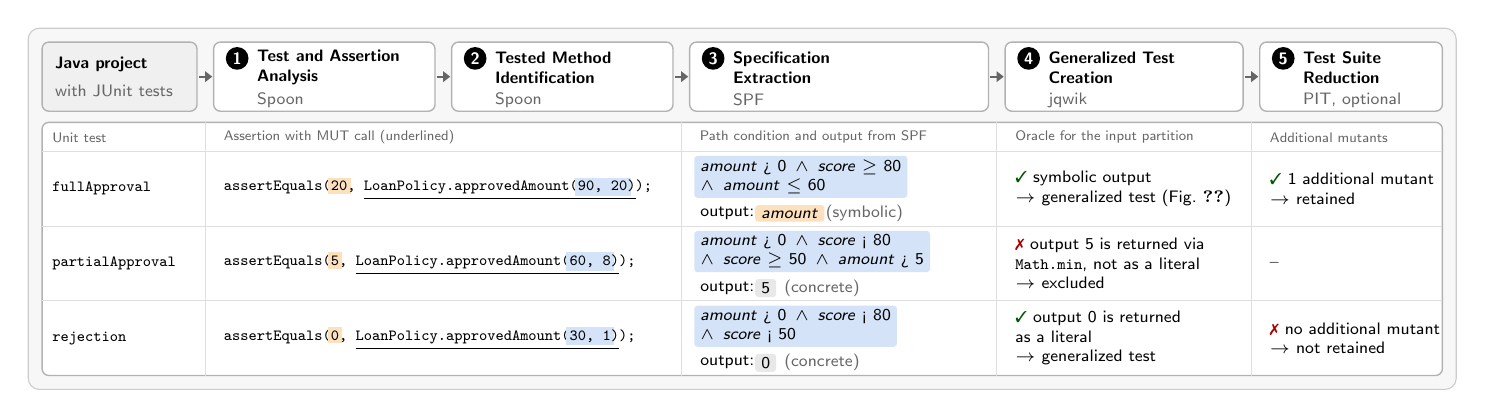
\begin{tikzpicture}[paperfig,
  sname/.style={anchor=west, inner sep=0pt, align=left, font=\sffamily\bfseries\fontsize{6.3}{7.2}\selectfont},
  tool/.style={tag, text=black!60},
  colhdr/.style={anchor=west, inner sep=0pt, font=\sffamily\fontsize{5.4}{6.3}\selectfont, text=black!60},
  cell/.style={anchor=west, inner sep=0pt, align=left, font=\sffamily\fontsize{5.7}{7.0}\selectfont},
  pc/.style={anchor=west, align=left, inner xsep=2.2pt, inner ysep=1.5pt, rounded corners=1.2pt, fill=inhl,
    font=\sffamily\fontsize{5.7}{6.8}\selectfont},
  outval/.style={anchor=west, inner xsep=2.2pt, inner ysep=1.3pt, rounded corners=1.2pt,
    font=\sffamily\fontsize{5.7}{6.8}\selectfont},
  rowcode/.style={anchor=west, inner sep=0pt, font=\fontfamily{lmtt}\fontsize{5.6}{6.7}\selectfont},
  nextstage/.style={-{Triangle[length=2.6pt, width=3.8pt]}, line width=0.8pt, black!60},
  guide/.style={black!13, line width=0.3pt},
]
\draw[rounded corners=4pt, fill=black!3, draw=black!20, line width=0.4pt] (0,0) rectangle (516,-130.5);

% The input and the five stages with the tool that each stage uses
% Source: sections/03-approach-00-intro.tex of the Teralizer paper (the figure of the five-stage pipeline and
% the tools that the stages build on), and sections/03-approach-05-reduction.tex of that paper (Stage 5 is
% optional)
\draw[panel, fill=black!6] (5,-5) rectangle (61,-30);
\node[sname] at (9.5,-13.2) {Java project};
\node[tool] at (9.5,-22.6) {with JUnit tests};
\foreach \x/\w/\n/\name/\uses in {
    67/80/1/{Test and Assertion\\Analysis}/Spoon,
    153/80/2/{Tested Method\\Identification}/Spoon,
    239/108/3/{Specification\\Extraction}/SPF,
    353/86/4/{Generalized Test\\Creation}/jqwik,
    445/66/5/{Test Suite\\Reduction}/{PIT, optional}} {
  \draw[panel] (\x,-5) rectangle (\x+\w,-30);
  \node[num] at (\x+8.5,-10.9) {\n};
  \node[sname] at (\x+15.5,-14.3) {\name};
  \node[tool] at (\x+15.5,-26) {\uses};
}
\foreach \x in {61.7, 147.7, 233.7, 347.7, 439.7} \draw[nextstage] (\x,-17.5) -- (\x+4.8,-17.5);

% The results of the stages for the three unit tests
\draw[panel] (5,-34) rectangle (511,-125.5);
\draw[guide] (5,-44.5) -- (511,-44.5);
\foreach \y in {-71.5, -98.5} \draw[guide] (5,\y) -- (511,\y);
\foreach \x in {64, 236, 350, 442} \draw[guide] (\x,-34) -- (\x,-125.5);
\node[colhdr] at (8.5,-39.5) {Unit test};
\node[colhdr] at (70.5,-39.5) {Assertion with MUT call (underlined)};
\node[colhdr] at (242.5,-39.5) {Path condition and output from SPF};
\node[colhdr] at (356.5,-39.5) {Oracle for the input partition};
\node[colhdr] at (448.5,-39.5) {Additional mutants};

% Source: demo/loan/src/test/java/bank/LoanPolicyTest.java (lines 8 to 16) for the tests and their assertions,
% demo/output/outcomes.txt for the MUT, the kind of output and the outcome of Stage 4,
% demo/output/specs/*.symbolic.input.json for the path conditions, *.symbolic.output.json and
% *.concrete.output.json for the outputs, lines 9 and 10 of demo/loan/src/main/java/bank/LoanPolicy.java for
% how the method returns the two concrete outputs, and demo/output/mutants.txt for the mutant that only the
% generalized test of fullApproval detects. Whether a test is retained follows from the rule of Stage 5 in
% sections/03-approach-05-reduction.tex of the Teralizer paper.

% fullApproval
\node[rowcode] at (8.5,-58) {fullApproval};
\node[rowcode] at (70.5,-58) {assertEquals(\slip{outhl}{20}, \underline{LoanPolicy.approvedAmount(\slip{inhl}{90, 20})});};
\node[pc] at (240.5,-53.7) {\textit{amount} > 0 \,$\land$\, \textit{score} $\ge$ 80\\$\land$\, \textit{amount} $\le$ 60};
\node[cell] at (242.7,-66.9) {output:};
\node[outval, fill=outhl] at (262.5,-66.9) {\textit{amount}};
\node[cell, text=black!60] at (288,-66.9) {(symbolic)};
\node[cell] at (356.5,-58) {\textcolor{green!35!black}{\ding{51}}\ symbolic output\\$\rightarrow$ generalized test (Fig.~\ref{fig:idea})};
\node[cell] at (448.5,-58) {\textcolor{green!35!black}{\ding{51}}\ 1 additional mutant\\$\rightarrow$ retained};

% partialApproval
\node[rowcode] at (8.5,-85) {partialApproval};
\node[rowcode] at (70.5,-85) {assertEquals(\slip{outhl}{5}, \underline{LoanPolicy.approvedAmount(\slip{inhl}{60, 8})});};
\node[pc] at (240.5,-80.7) {\textit{amount} > 0 \,$\land$\, \textit{score} < 80\\$\land$\, \textit{score} $\ge$ 50 \,$\land$\, \textit{amount} > 5};
\node[cell] at (242.7,-93.9) {output:};
\node[outval, fill=black!9] at (262.5,-93.9) {5};
\node[cell, text=black!60] at (273,-93.9) {(concrete)};
\node[cell] at (356.5,-85) {\textcolor{red!65!black}{\ding{55}}\ output 5 is returned via\\\code{Math.min}, not as a literal\\$\rightarrow$ excluded};
\node[cell, text=black!60] at (448.5,-85) {--};

% rejection
\node[rowcode] at (8.5,-112) {rejection};
\node[rowcode] at (70.5,-112) {assertEquals(\slip{outhl}{0}, \underline{LoanPolicy.approvedAmount(\slip{inhl}{30, 1})});};
\node[pc] at (240.5,-107.7) {\textit{amount} > 0 \,$\land$\, \textit{score} < 80\\$\land$\, \textit{score} < 50};
\node[cell] at (242.7,-120.9) {output:};
\node[outval, fill=black!9] at (262.5,-120.9) {0};
\node[cell, text=black!60] at (273,-120.9) {(concrete)};
\node[cell] at (356.5,-112) {\textcolor{green!35!black}{\ding{51}}\ output 0 is returned\\as a literal\\$\rightarrow$ generalized test};
\node[cell] at (448.5,-112) {\textcolor{red!65!black}{\ding{55}}\ no additional mutant\\$\rightarrow$ not retained};
\end{tikzpicture}

% Source: the sources that figures/pipeline.tex names for the stages and for the results
\caption{The five stages of \Teralizer{} with the tools that they use, and their results for the three unit tests of the running example.}
\label{fig:pipeline}
\end{figure*}

\section{Introduction}
\label{sec:introduction}

% Source: sections/01-introduction.tex of the Teralizer paper for the limitation of unit tests, demo/loan for the
% example, demo/refactoring/LoanPolicy.java for the refactoring, and demo/output/regression.txt for the result of
% the unit tests after it
Unit tests are widely used to detect regressions, i.e., unintended changes in program behavior.
Since a conventional unit test validates the method under test (MUT) only for specific input-output pairs, regressions that affect other inputs remain undetected.
Fig.~\ref{fig:idea} shows an example.
The method \code{approvedAmount} approves loans of up to \code{FULL} for applicants with a credit score of at least 80, and the unit test \code{fullApproval} validates this behavior for a score of 90 and a requested amount of 20.
A refactoring that merges the two calls of \code{Math.min} unintentionally changes the condition \code{score >= 80} to \code{score > 80}.
Applicants with a score of 80 are thereby approved for at most \code{PARTIAL} instead of \code{FULL}, but the unit test \code{fullApproval} still passes.

% Source: sections/02-background.tex of the Teralizer paper (Property-Based Testing as Target Representation)
Property-based testing (PBT)~\cite{claessen_2000_quickcheck} addresses this limitation by validating properties across many inputs that are produced by generators.
In the example, a property-based test that validates the approved amount for all scores of at least 80 detects the regression.
However, writing property-based tests requires developers to identify suitable properties and to define generators with appropriate constraints, which practitioners find challenging and which limits the adoption of PBT~\cite{goldstein_2024_pbt_practice}.

% Source: sections/01-introduction.tex and sections/03-approach-00-intro.tex (Concepts and Algorithm) of the Teralizer
% paper, and demo/output/regression.txt for the detected regression
In this paper, we present \Teralizer{}, a tool that automatically generalizes JUnit tests into property-based jqwik~\cite{link_2022_jqwik} tests based on the approach of our previous work~\cite{glock_2025_teralizer}.
Through single-path symbolic analysis with Symbolic PathFinder (SPF)~\cite{pasareanu_2013_symbolic}, \Teralizer{} extracts from the execution of a unit test a \emph{path condition}, which characterizes all inputs that follow the same execution path as the original inputs, and a \emph{symbolic output expression}, which computes the expected output for these inputs.
It then creates a property-based test that generates inputs satisfying the path condition and uses the symbolic output expression as the expected value of the original assertion.
In Fig.~\ref{fig:idea}, this generalized test detects the regression that the unit test misses.

% Source: main.bib (glock_2025_teralizer)
The approach and its evaluation are described in detail in~\cite{glock_2025_teralizer}, while this paper focuses on the implementation and the usage of the tool.
% Source: LICENSE-MIT in the Teralizer repository. 10.5281/zenodo.17950380 is the concept DOI of the Zenodo
% record, which resolves to its latest version (10.5281/zenodo.18242626 in the README of the repository).
\Teralizer{} is open source under the MIT license,\footnote{\url{https://github.com/glockyco/Teralizer}} with a replication package on Zenodo~\cite{glock_2026_replication}.

\section{Overview of \Teralizer{}}
\label{sec:approach}

% Source: README.md of the Teralizer repository, and sections/03-approach-00-intro.tex of the Teralizer paper
% (the five stages, recorded exclusions, implementation scope and automation), and
% sections/03-approach-04-generalization.tex of that paper (one new test class per assertion)
\Teralizer{} is implemented in Java and takes a Maven or Gradle project with JUnit~3, 4, or~5 tests as input, to which it adds the generalized tests as jqwik test classes.
Fig.~\ref{fig:pipeline} shows the five stages of its fully automated pipeline~\cite{glock_2025_teralizer} and their results for the three unit tests of the running example.
Tests and assertions that a stage cannot process are excluded from the subsequent stages, and the reasons are recorded.

% Source: sections/03-approach-01-test-analysis.tex and sections/03-approach-02-mut-identification.tex of the
% Teralizer paper, and sections/03-approach-00-intro.tex of that paper (scope of exactness) for the supported types
\runin{Stages 1 and 2}
\Teralizer{} executes the test suite and analyzes all passing tests with Spoon~\cite{pawlak_2016_spoon}.
Stage~1 identifies the assertions that \Teralizer{} can generalize, which currently are equality, Boolean, and exception assertions of JUnit and equality assertions of Hamcrest.
Stage~2 identifies the MUT call of each assertion, i.e., the method call whose result the assertion validates.
For this purpose, a data-flow analysis traces the asserted value back to the method call that produced it.
If the analysis does not yield a unique call, a ranking heuristic selects one of the preceding calls based on its parameter and return types, its class, its name, and its distance to the assertion.
Arguments of primitive types, their boxed types, and strings become the inputs of the generalized test.

% Source: sections/03-approach-03-spec-extraction.tex of the Teralizer paper, and demo/output/specs for the outputs
% of the three tests (symbolic.output.json and concrete.output.json)
\runin{Stage 3}
\Teralizer{} executes each test with SPF using single-path symbolic analysis, which treats these arguments as symbolic values while it follows the execution path of the original inputs and therefore requires no constraint solving.
SPF adds the condition of each taken branch that depends on a symbolic value to the path condition.
When the MUT returns, \Teralizer{} records the path condition and the output as the input/output specification.
For \code{fullApproval}, the output is the symbolic expression $\mathit{amount}$, whereas SPF provides only the concrete outputs 5 and~0 for the other two tests.

% Source: sections/03-approach-04-generalization.tex of the Teralizer paper (Transformation Process, widening
% refusals), teralizer.generalization.WideningLicense in the Teralizer repository, and demo/output/outcomes.txt and
% demo/output/excluded.txt for the two tests
\runin{Stage 4}
\Teralizer{} creates a jqwik test class with a property-based version of the original test (Fig.~\ref{fig:idea}), in which the arguments of the MUT call are replaced with generated parameters and the expected value of the assertion with the output of the specification.
The output therefore has to be a valid oracle for all inputs of the input partition, which holds for a symbolic output expression.
A concrete output is not necessarily constant for the input partition, because SPF also provides only a concrete output when it cannot track the dependence of the output on the inputs, e.g., for outputs that are accumulated in input-dependent loops~\cite{glock_2025_teralizer}.
\Teralizer{} therefore uses a concrete output only if the MUT directly returns a literal, as in \code{rejection} (\code{return 0}).
In \code{partialApproval}, the constant is returned via \code{Math.min}, which the current implementation does not recognize as constant, so that the assertion is excluded.

% Source: sections/03-approach-04-generalization.tex of the Teralizer paper (Three-Variant Design, Constraint-Aware
% Generation, validation of generalized tests), and demo/output/inputs/2.IMPROVED_200_TRIES.values.tsv for the
% inputs that the generalized test of fullApproval tries
The parameters are generated according to one of two strategies.
\Naive{} generates random values and applies the path condition as a filter.
\Improved{} additionally encodes constraints that compare a parameter with a constant or with another parameter in the generators, which reduces the number of rejected inputs and enables jqwik to generate inputs at the boundaries of the input partition, such as the score of 80 that reveals the regression in Fig.~\ref{fig:idea}.
The figure shows these constraints as jqwik annotations, whereas the generated code implements them in a supplier class.
A generalized test first executes the original inputs and then generated inputs, up to a configurable number of inputs per test (tries).
Generalized tests that fail for the current implementation are excluded.

% Source: sections/03-approach-05-reduction.tex of the Teralizer paper, demo/output/mutants.txt, and line 8 of
% demo/loan/src/main/java/bank/LoanPolicy.java for the mutated condition
\runin{Stage 5}
This optional stage applies mutation testing with PIT~\cite{coles_2016_pit} and retains a generalized test only if it detects at least one mutant that the original test suite does not detect.
In the example, this holds for \code{fullApproval}, whose generalized test detects the mutant that changes \mbox{\code{score >= 80}} to \mbox{\code{score > 80}}, i.e., the fault that the refactoring of Fig.~\ref{fig:idea} introduces.

\begin{figure}[t]
% Source: demo/output/console.txt, which holds what scripts/try-example.sh of the Teralizer repository prints for
% the example. The excerpt marks the lines and the parts of lines that it leaves out with [...].
\begin{lstlisting}[style=console]
==> Outcome of each assertion that reached generalization
      test       | tested_method  | generalized |              reason
-----------------+----------------+-------------+----------------------------------
 fullApproval    | approvedAmount | t           |
 partialApproval | approvedAmount | f           | NULL_CONCRETE_OUTPUT_NOT_LITERAL
 rejection       | approvedAmount | t           |
[...]
==> Running all tests against the refactored example
[INFO] Tests run: 3, Failures: 0, Errors: 0, Skipped: 0 -- in bank.LoanPolicyTest
    expected: <60> but was: <5>
tries = 4                     | # of calls to property
  arg0: TestParameters{score=80,amount=60}
[ERROR] Tests run: 1, Failures: 1, [...] -- in [...]_Generalized_fullApproval_2_Test
[...]
\end{lstlisting}
\caption{Output of \code{scripts/try-example.sh} for the example (abridged).}
\label{fig:output}
\end{figure}

\section{Usage}
\label{sec:usage}

% Source: README.md of the Teralizer repository (Try it on an example)
\Teralizer{} is executed in a Docker container.
On a machine with Bash, Git LFS, and Docker, the following commands build the image in a clone of the repository and apply \Teralizer{} to the running example:
\begin{lstlisting}[style=code]
git lfs pull
git submodule update --init --recursive jpf-symbc
docker build -t teralizer .
scripts/try-example.sh
\end{lstlisting}
% Source: scripts/try-example.sh in the Teralizer repository, and demo/output/console.txt for what it prints
\noindent The script \code{try-example.sh} runs the pipeline on a copy of the example and prints the results (Fig.~\ref{fig:output}).
It reports for each assertion that reaches Stage~4 whether a generalized test was created or why the assertion was excluded, the mutants that the original and the generalized test suite detect, and the paths of the generalized test classes.
% Source: demo/output/regression.txt for the results
It then applies the refactoring of Fig.~\ref{fig:idea} and executes all tests.
The three original tests pass, whereas the generalized test of \code{fullApproval} fails at the fourth try and reports the failing input together with the expected and the actual output.
% Source: demo/output/run.txt for the runtime, and demo/output/machine.txt for the machine
Processing the example takes less than two minutes on a laptop (Intel Core Ultra~7 265H, 16\,GB of memory assigned to Docker).

% Source: README.md of the Teralizer repository (Try it on an example) and scripts/try-example.sh for other projects,
% and demo/loan.conf for the configuration
For another project, the script takes the project directory as its argument.
The project has to build with Java~8, which SPF requires, and use Maven or Gradle with JUnit~3, 4, or~5.
% Source: demo/loan.conf (lines 3 to 5)
The script works on a copy of the project and uses the configuration file of the running example, which specifies the generalization strategy and the number of tries per generalized test:
\begin{lstlisting}[style=code]
teralizer.generalizations.IMPROVED_200_TRIES {
  algorithm = "IMPROVED", jqwik.tries = 200
}
\end{lstlisting}

% Source: sections/03-approach-04-generalization.tex of the Teralizer paper (one new test class per assertion),
% demo/output/generated for the classes, and demo/output/adoption.txt for a run of all tests of the example with jqwik
% as the only added dependency
\Teralizer{} adds each generalized test as a separate jqwik test class to the package of the original test class and does not modify existing tests.
The generalized tests are executed on the JUnit Platform.
In the running example, adding jqwik as a test dependency is sufficient to execute them together with the original tests via \code{mvn test}.
% Source: sections/03-approach-00-intro.tex of the Teralizer paper (every exclusion is recorded with its reason),
% and scripts/try-example.sh for the database and its queries
The results of all stages and the reasons for all exclusions are stored in a PostgreSQL database.

\begin{figure}[t]
\centering
% Fig. 2: mutation scores and total runtimes of EvoSuite alone and of EvoSuite followed by Teralizer,
% drawn at the column width of IEEEtran conference papers (252 pt).
% Source: the Pareto points of analysis/reports/rq4.md in the Teralizer repository (detection in
% percent, runtime in seconds), and for EvoSuite with 60 s on EqBench, which is not on the front,
% sections/04-evaluation-07-rq4.tex of the Teralizer paper (51.6% in 55,075 s). The same section
% gives the two comparisons that the left plot marks. The layout follows
% talks/components/ParetoPlot.vue of the PhD seminar talk.
% Coordinates are (runtime in 1000 s, mutation score in percent). Each scope maps them to its plot area.
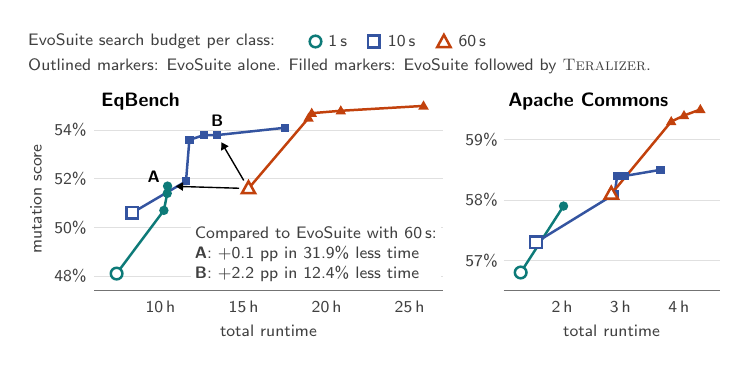
\begin{tikzpicture}[x=1pt, y=1pt, font=\sffamily\fontsize{6.2}{7.2}\selectfont,
  grid/.style={black!12, line width=0.3pt},
  axis/.style={black!55, line width=0.4pt},
  tick/.style={inner sep=0pt, text=black!75},
  name/.style={inner sep=0pt, anchor=north west, font=\sffamily\bfseries\fontsize{6.6}{7.6}\selectfont},
  chain/.style={line width=0.9pt, line join=round},
  b1/.style={color=effone}, b10/.style={color=efften}, b60/.style={color=effsixty},
  alone/.style={fill=white, line width=0.9pt},
  gain/.style={black, line width=0.5pt, -{Triangle[length=2.6pt, width=3pt]}, shorten <=3.4pt, shorten >=3pt},
  note/.style={inner sep=0pt, font=\sffamily\bfseries\fontsize{6.2}{7}\selectfont},
  dot/.pic={\fill (0,0) circle[radius=1.7pt];},
  sq/.pic={\fill (-1.5pt,-1.5pt) rectangle (1.5pt,1.5pt);},
  tri/.pic={\fill (-1.9pt,-1.3pt) -- (1.9pt,-1.3pt) -- (0,2pt) -- cycle;},
]
% Legend
% Source: the columns EvoSuite and Teralizer of the two tables of Pareto points in analysis/reports/rq4.md
\useasboundingbox (0,-5) rectangle (252,111);
\node[tick, anchor=west] at (0,106) {EvoSuite search budget per class:};
\draw[b1, alone] (104,106) circle[radius=2.1pt];
\node[tick, anchor=west] at (108.5,106) {1\,s};
\draw[b10, alone] (123,103.9) rectangle (127.2,108.1);
\node[tick, anchor=west] at (130,106) {10\,s};
\draw[b60, alone] (148,104) -- (152.8,104) -- (150.4,108.4) -- cycle;
\node[tick, anchor=west] at (155.5,106) {60\,s};
\node[tick, anchor=west] at (0,97) {Outlined markers: EvoSuite alone. Filled markers: EvoSuite followed by \Teralizer{}.};

\node[tick, rotate=90] at (3,49) {mutation score};

% EqBench: 6 h to 27 h on 126 pt, 47.4% to 55.6% on 72 pt
% Source: the table "Pareto points for eqbench" of analysis/reports/rq4.md, and
% sections/04-evaluation-07-rq4.tex of the Teralizer paper for EvoSuite with 60 s (51.6% in 55,075 s)
\begin{scope}[shift={(-12,-400.2)}, x=1.6667pt, y=8.7805pt]
  \foreach \det in {48, 50, 52, 54} {
    \draw[grid] (21.6,\det) -- (97.2,\det);
    \node[tick, anchor=east] at (20.1,\det) {\det\%};}
  \draw[axis] (21.6,47.4) -- (97.2,47.4);
  \foreach \hours/\ks in {10/36, 15/54, 20/72, 25/90}
    \node[tick, anchor=north] at (\ks,46.99) {\hours\,h};
  \node[tick, anchor=north] at (59.4,46.0) {total runtime};
  \node[name] at (23,55.55) {EqBench};

  \draw[chain, b1] (26.479,48.1) -- (36.728,50.7) -- (37.457,51.4) -- (37.532,51.7);
  \draw[chain, b10] (29.861,50.6) -- (41.525,51.9) -- (42.256,53.6) -- (45.398,53.8) -- (48.269,53.8) -- (62.938,54.1);
  \draw[chain, b60] (55.075,51.6) -- (68.093,54.5) -- (68.782,54.7) -- (75.081,54.8) -- (93.017,55.0);
  \foreach \point in {(36.728,50.7), (37.457,51.4), (37.532,51.7)} \pic[b1] at \point {dot};
  \foreach \point in {(41.525,51.9), (42.256,53.6), (45.398,53.8), (48.269,53.8), (62.938,54.1)} \pic[b10] at \point {sq};
  \foreach \point in {(68.093,54.5), (68.782,54.7), (75.081,54.8), (93.017,55.0)} \pic[b60] at \point {tri};
  \draw[b1, alone] (26.479,48.1) circle[radius=2.1pt];
  \draw[b10, alone] (29.861,50.6) +(-2.1pt,-2.1pt) rectangle +(2.1pt,2.1pt);
  \draw[b60, alone] (55.075,51.6) +(-2.4pt,-1.7pt) -- +(2.4pt,-1.7pt) -- +(0,2.6pt) -- cycle;

  % The two generalized test suites that the text compares with EvoSuite at 60 s
  % Source: sections/04-evaluation-07-rq4.tex of the Teralizer paper (0.1 percentage points higher detection with
  % 31.9% lower runtime, and 2.2 percentage points in 12.4% less runtime)
  \draw[gain] (55.075,51.6) -- (37.532,51.7);
  \draw[gain] (55.075,51.6) -- (48.269,53.8);
  \node[note, anchor=south east] at ([xshift=-2.6pt, yshift=1pt]37.532,51.7) {A};
  \node[note, anchor=south] at ([yshift=2.8pt]48.269,53.8) {B};
  \node[tick, anchor=south east, align=left, fill=white, inner sep=1.5pt] at (96.9,47.57)
    {Compared to EvoSuite with 60\,s:\\\textbf{A}: +0.1 pp in 31.9\% less time\\\textbf{B}: +2.2 pp in 12.4\% less time};
\end{scope}

% Apache Commons: 1 h to 4.7 h on 78 pt, 56.5% to 59.8% on 72 pt
% Source: the table "Pareto points for commons-utils" of analysis/reports/rq4.md
\begin{scope}[shift={(150.92,-1216.73)}, x=5.8559pt, y=21.818pt]
  \foreach \det in {57, 58, 59} {
    \draw[grid] (3.6,\det) -- (16.92,\det);
    \node[tick, anchor=east] at (3.27,\det) {\det\%};}
  \draw[axis] (3.6,56.5) -- (16.92,56.5);
  \foreach \hours/\ks in {2/7.2, 3/10.8, 4/14.4}
    \node[tick, anchor=north] at (\ks,56.335) {\hours\,h};
  \node[tick, anchor=north] at (10.26,55.936) {total runtime};
  \node[name] at (3.85,59.777) {Apache Commons};

  \draw[chain, b1] (4.649,56.8) -- (7.294,57.9);
  \draw[chain, b10] (5.597,57.3) -- (10.445,58.1) -- (10.603,58.4) -- (11.082,58.4) -- (13.270,58.5);
  \draw[chain, b60] (10.240,58.1) -- (13.939,59.3) -- (14.728,59.4) -- (15.736,59.5);
  \pic[b1] at (7.294,57.9) {dot};
  \foreach \point in {(10.445,58.1), (10.603,58.4), (11.082,58.4), (13.270,58.5)} \pic[b10] at \point {sq};
  \foreach \point in {(13.939,59.3), (14.728,59.4), (15.736,59.5)} \pic[b60] at \point {tri};
  \draw[b1, alone] (4.649,56.8) circle[radius=2.1pt];
  \draw[b10, alone] (5.597,57.3) +(-2.1pt,-2.1pt) rectangle +(2.1pt,2.1pt);
  \draw[b60, alone] (10.240,58.1) +(-2.4pt,-1.7pt) -- +(2.4pt,-1.7pt) -- +(0,2.6pt) -- cycle;
\end{scope}
\end{tikzpicture}

% Source: analysis/reports/rq4.md of the Teralizer repository (the Pareto points with their EvoSuite budgets,
% generalization strategies and tries), and sections/04-evaluation-07-rq4.tex of the Teralizer paper
\caption{Mutation scores and total runtimes of EvoSuite alone and followed by \Teralizer{}~\cite{glock_2025_teralizer}. Lines connect each EvoSuite test suite with the Pareto-optimal test suites that \Teralizer{} creates from it (pp: percentage points).}
\label{fig:efficiency}
\end{figure}

\section{Evaluation}
\label{sec:evaluation}

% Source: sections/04-evaluation-02-framework.tex of the Teralizer paper
The evaluation in~\cite{glock_2025_teralizer} uses test suites that EvoSuite~\cite{fraser_2011_evosuite} generates with search budgets of 1\,s, 10\,s, and 60\,s per class for the EqBench benchmark~\cite{badihi_2021_eqbench} and for numeric utility classes of Apache Commons~\cite{apache_commons}, the developer-written tests of the same classes, and 584 open-source projects from the RepoReapers dataset~\cite{munaiah_2017_reporeapers}.
Mutation scores are measured with PIT.

% Source: macros TzEffectiveness* in tables/generated/macros.tex of the Teralizer paper, and
% sections/04-evaluation-04-rq1.tex of that paper for what the ranges span. tables/generated/tab-detections-per-mutator.tex
% of that paper for the mutation operators with the largest increases (Math with both strategies, and
% ConditionalsBoundary as the second largest with Improved), and demo/output/mutants.txt for the mutation
% operator of the mutant that the generalized test of the example detects.
\runin{Effectiveness}
Generalization increases the mutation scores of the EvoSuite-generated test suites by 1.22--3.93 percentage points for EqBench and by 0.82--1.33 percentage points for Apache Commons, depending on the search budget, the generalization strategy, and the number of tries.
For the developer-written tests, which already achieve a mutation score of 80.35\%, the increase is 0.05--0.07 percentage points.
The detection rate increases most for mutants of arithmetic operations and, with \Improved{}, for mutants of conditional boundaries, such as the mutant of the running example.

% Source: Pareto points in analysis/reports/rq4.md of the Teralizer repository, and sections/04-evaluation-07-rq4.tex
% of the Teralizer paper for the two comparisons with EvoSuite with 60 s on EqBench, for Apache Commons, and for
% the share of Stage 5 in the processing time. sections/04-evaluation-06-rq3.tex of that paper for the 21,478
% created generalized tests, of which test suite reduction retains 1,555 (7.2%).
\runin{Efficiency}
For EqBench, EvoSuite with a search budget of 1\,s followed by \Teralizer{} (A~in Fig.~\ref{fig:efficiency}) achieves a 0.1~percentage points higher mutation score than EvoSuite with a search budget of 60\,s in 31.9\% less total runtime.
With a search budget of 10\,s (B), this combination achieves a 2.2~percentage points higher mutation score in 12.4\% less time.
For Apache Commons, all test suites of EvoSuite are Pareto-optimal, but generalization achieves higher mutation scores than EvoSuite alone (59.5\% vs.\ 58.1\%).
Stage~5 takes 59.1--95.7\% of the processing time of \Teralizer{} and retains 1,555 of the 21,478 generalized tests (7.2\%).

% Source: macros TzRealworld* in tables/generated/macros.tex of the Teralizer paper, sections/05-discussion.tex of
% that paper (When and Why Generalization Fails) for the main causes, and tables/generated/tab-exclusions-breakdown.tex
% of that paper for the 47.8% of the assertions in the EqBench and Apache Commons test suites
\runin{Applicability}
The current prototype of \Teralizer{} is less successful for real-world projects.
Of the 584 RepoReapers projects, 85 (14.6\%) complete all five stages, which yields 1,435 generalized tests.
Across all projects, 3.8\% of the assertions pass the first three stages, compared with 47.8\% for EqBench and Apache Commons.
The other assertions are excluded mainly because no MUT call can be identified or because the parameters or the return value of the MUT have unsupported types.
In Stage~4, 61.6\% of the generalization attempts are excluded for lack of a valid oracle, 77.4\% of them because of a concrete output that the MUT does not return as a literal, as in \code{partialApproval}.

\section{Limitations and Future Work}
\label{sec:outlook}

% Source: sections/01-introduction.tex (regression detection) and sections/03-approach-00-intro.tex (scope of
% exactness) of the Teralizer paper
Since the oracles of the generalized tests are derived from the implementation, generalized tests detect behavioral changes in later versions, but not faults that are already present in the analyzed version.
Moreover, single-path symbolic analysis requires pure MUTs, i.e., deterministic MUTs without side effects that depend only on their parameters~\cite{glock_2025_teralizer}.

% Source: sections/03-approach-00-intro.tex (implementation scope) and sections/05-discussion.tex (Improving
% Applicability, Type Support) of the Teralizer paper, chapters/06-reflections/04-directions.tex of the first
% author's PhD thesis (SPF is designed to construct exact models for solver-backed verification), and the comment
% of the first author on the limitations of the first draft (docs/author-review.md at commit 1e80f94)
The applicability of \Teralizer{} is mainly limited by the underlying symbolic analysis.
SPF requires Java~8.
Since it constructs exact symbolic models for constraint solving~\cite{pasareanu_2013_symbolic}, it supports only inputs and outputs of primitive types, their boxed types, and strings.
Test generalization has weaker requirements than constraint solving, because a generator that covers only a subset of an input partition reduces the number of tested inputs, but does not cause spurious test failures~\cite{glock_2025_teralizer}.
We therefore plan to extend the symbolic analysis beyond what is required for constraint solving, e.g., with approximate models for arrays, objects, and further string operations.

% Source: demo/output/generated/_LoanPolicyTest_Generalized_fullApproval_2_Test.java (412 lines, of which the
% test method takes 7, the parameter class 13, and the generators and the recording of inputs the rest), and the
% same comment of the first author
So far, we have not focused on the presentation of the generalized tests.
For example, the generated test class of \code{fullApproval} comprises 412 lines of code, most of which implement the generators and record the tested inputs for the evaluation, compared to six lines of the simplified version in Fig.~\ref{fig:idea}.
In future work, we plan to make the generalized tests easier to understand and to maintain for practitioners.

\section{Related Work}
\label{sec:related-work}

% Source: sections/02-background.tex (Test Amplification and Generalization) and sections/01-introduction.tex of the
% Teralizer paper, the abstract of the cited literature study for what test amplification does, and comment 5 of the
% first author's review of the rewrite (docs/author-review.md at commit 76135d4)
Test generalization is a form of test amplification~\cite{danglot_2019_snowballing}, which enhances existing tests.
Test generation tools such as EvoSuite~\cite{fraser_2011_evosuite} instead infer test scenarios and assertions from the observed behavior of the implementation, which risks overfitting the implementation~\cite{barr_2015_oracle}.
The setup code and assertions of developer-written tests encode knowledge about the intended behavior that the implementation itself does not contain, which makes their generalized tests less likely to overfit the implementation.
Both techniques can be combined by generalizing generated tests, as in Section~\ref{sec:evaluation}.

% Source: sections/01-introduction.tex and sections/06-related-work.tex of the Teralizer paper, and analysis/reports/rq0.md
% of the Teralizer repository for the projects with generalized tests
To our knowledge, JARVIS~\cite{peleg_2018_jarvis} is the only other tool that automatically generalizes unit tests into property-based tests.
It infers properties from groups of similar tests based on predefined abstraction templates and does not analyze the implementation.
\Teralizer{} creates generalized tests in 9 of the 12 projects of the JARVIS evaluation, whereas the published JARVIS results cover 2 projects~\cite{glock_2025_teralizer}.
Approaches that generate parameterized unit tests start from tests without assertions~\cite{fraser_2011_generating_put} or use values observed at runtime~\cite{tiwari_2024_proze} and do not generalize oracles beyond these values.
Large language models generate property-based tests without existing tests, but their generators and assertions can be invalid or unsound~\cite{vikram_2024_pbt}.

\section{Conclusion}
\label{sec:conclusion}

% Source: sections/03-approach-00-intro.tex of the Teralizer paper, and README.md of the Teralizer repository
We presented \Teralizer{}, a tool that automatically generalizes JUnit tests into property-based jqwik tests based on single-path symbolic analysis.
The generalized tests validate the original assertions across the tested input partitions and thereby detect regressions that the original tests miss.

\section*{Acknowledgment}
% Source: the acknowledgment of the Teralizer paper (main.tex)
This research was funded in whole or in part by the Austrian Science Fund (FWF) 10.55776/P36698.
For open access purposes, the author has applied a CC BY public copyright license to any author accepted manuscript version arising from this submission.
% Source: SCCH's funding text and the AI disclosure of the authors' other papers.
% SCCH asks for its full funding text and allows this short one when a paper runs out of space.
The research reported in this paper has been partly funded by BMIMI, BMWET, and the State of Upper Austria in the frame of the SCCH competence center INTEGRATE (FFG grant no.~892418) part of the FFG COMET Competence Centers for Excellent Technologies Programme.
We used OpenAI GPT, Anthropic Claude, and Google Gemini models to assist with writing, coding, and literature search.
The authors reviewed and refined the generated material and take full responsibility for the final manuscript.

\bibliographystyle{IEEEtran}
\bibliography{main}

\end{document}
